\documentclass[11pt]{article}
\usepackage[margin=1in]{geometry}

% --- Figures / floats ---
\usepackage{graphicx}     % graphicx: provides \includegraphics
\usepackage{caption}      % caption: controls caption formatting
\usepackage{subcaption}   % subcaption: sub-figures support
\usepackage{placeins}     % placeins: provides \FloatBarrier to stop floats crossing barriers
\usepackage{float}        % float: provides [H] specifier if you want to force exact placement

\usepackage{amsmath}
\usepackage{hyperref}
\usepackage{parskip}

\captionsetup{labelfont=bf,font=small}
\graphicspath{{../figures/}}

\title{Spam Email Classification Using Naive Bayes with Clustering-Enhanced Features}
\author{Tom Hines\\Quantifying the World\\Southern Methodist University}
\date{February 16, 2026}

\begin{document}
\maketitle

\section{Introduction}

This case study addresses email spam filtering using probabilistic classification: Naive Bayes with features built from TF-IDF vectorization and K-Means clustering. The SpamAssassin public corpus provides a realistic benchmark with an imbalanced class distribution (approximately 74\% ham and 26\% spam), which motivated the choice of Complement Naive Bayes. The pipeline uses only cross-validation for evaluation, with no train--test split, and all predictions are out-of-fold to avoid data leakage.

\section{Data and Preprocessing}

The dataset is assembled from five SpamAssassin categories (easy\_ham, easy\_ham\_2, hard\_ham, spam, spam\_2), yielding 9,353 emails parsed with Latin-1 encoding. Figure~\ref{fig:data} summarizes class distribution and content types (MIME). The 74--26 ham-to-spam imbalance is typical of real-world mail streams and was preserved throughout. 

Preprocessing extracts body text (and optionally subject) from single-part and multipart messages, stripping HTML to plain text. Normalization includes lowercasing, removal of URLs and email addresses, stripping non-alphanumeric characters, and collapsing whitespace; no imputation was applied (one email yielded an empty string after cleaning and was removed). The pipeline then applies stopword removal, a minimum token length, and a simple suffix stemmer. Feature creation is described in the next section. The final count sat at 9,352 samples, and the data is treated as a Bag-of-Words model for encoding.

\begin{figure}[!htbp]
\centering
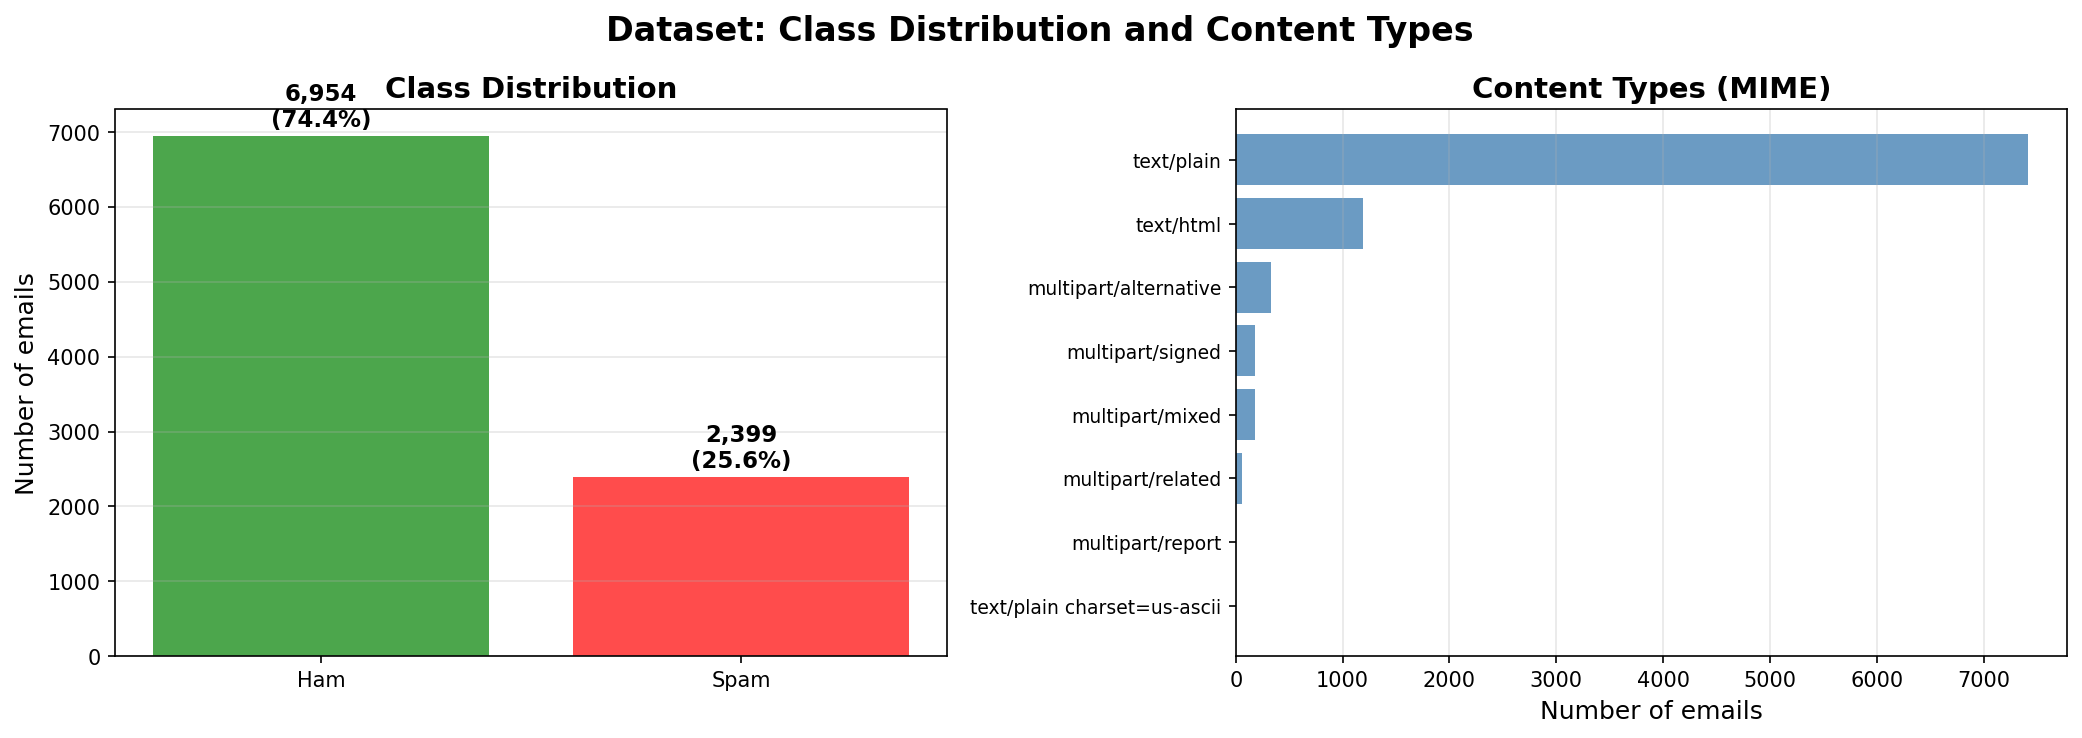
\includegraphics[width=0.85\textwidth]{00_class_and_content_distribution.png}
\caption{Class distribution (ham vs.\ spam) and distribution of MIME content types in the SpamAssassin dataset. The imbalance (74\% ham, 26\% spam) was preserved for training and evaluation.}
\label{fig:data}
\end{figure}

\FloatBarrier

\section{Feature Engineering and Clustering}

Features are built with TF-IDF vectorization (3,000 terms, min/max document frequency 2 and 0.95, unigrams and bigrams). TF-IDF emphasizes terms that are distinctive per document, which suits spam detection where phrases like ``free,'' ``click,'' and ``offer'' are telling. The resulting sparse matrix is combined with cluster-based features.

Clustering is used only as an unsupervised method (K-Means); no supervised use such as KNN was applied. The number of clusters was chosen by evaluating $k \in [2, 30]$ on a 3,000-point sample using inertia, silhouette score, and the Calinski--Harabasz index. Silhouette score was used as the primary criterion; it peaked at $k = 28$, which was selected to capture fine-grained thematic structure (e.g., different spam types and legitimate email genres). Mini-Batch K-Means was fit on the full BOW matrix; the assigned cluster for each email was one-hot encoded and these new features were concatenated with the original TF-IDF matrix to form a 3,028-dimensional feature set.

\section{Model and Validation}

Complement Naive Bayes was chosen because it is designed for imbalanced text: it estimates parameters from the complement of each class, reducing bias toward the majority class. Laplace smoothing ($\alpha = 1.0$) was applied. Evaluation used stratified 10-fold cross-validation so that each fold preserves the 74--26 class ratio. Predictions and class probabilities were obtained via \texttt{cross\_val\_predict}, ensuring every sample is predicted only when held out.

Fold accuracies ranged from 94.33\% to 97.11\% (mean 95.62\%, standard deviation 0.90\%), indicating stable generalization.

\section{Results}

All 9,352 samples were predicted out of fold (no sample was predicted by a model trained on it). The out-of-fold confusion matrix (Figure~\ref{fig:confusion}) shows 6,674 true negatives, 280 false positives, 130 false negatives, and 2,269 true positives. Table~\ref{tab:classification} presents the classification report: precision, recall, F1-score, and support for each class. The final accuracy across all folds of the CV is 95.62\%.

\begin{table}[!htbp]
\centering
\caption{Classification report (out-of-fold predictions).}
\label{tab:classification}
\begin{tabular}{lcccc}
\hline
Class & Precision & Recall & F1-score & Support \\
\hline
Ham (0)  & 0.9809 & 0.9597 & 0.9702 & 6954 \\
Spam (1) & 0.8902 & 0.9458 & 0.9171 & 2399 \\
\hline
Accuracy & \multicolumn{4}{c}{0.9562 (9352)} \\
\hline
\end{tabular}
\end{table}

The 280 false positives (ham predicted as spam) often correspond to legitimate promotional or newsletter-style emails that use commercial language (e.g., ``offer,'' ``sale'') or multiple links, which the model associates with spam. The 130 false negatives (spam predicted as ham) tend to be messages that mimic legitimate tone and formatting or carry little text. Examining these misses suggests that improvement within the current setup could come from richer handling of context (e.g., subject vs.\ body) or threshold tuning to trade off false positives against false negatives; the model ``fails'' on those cases mainly where the lexical and cluster signals overlap with the other class.

\begin{figure}[!htbp]
\centering
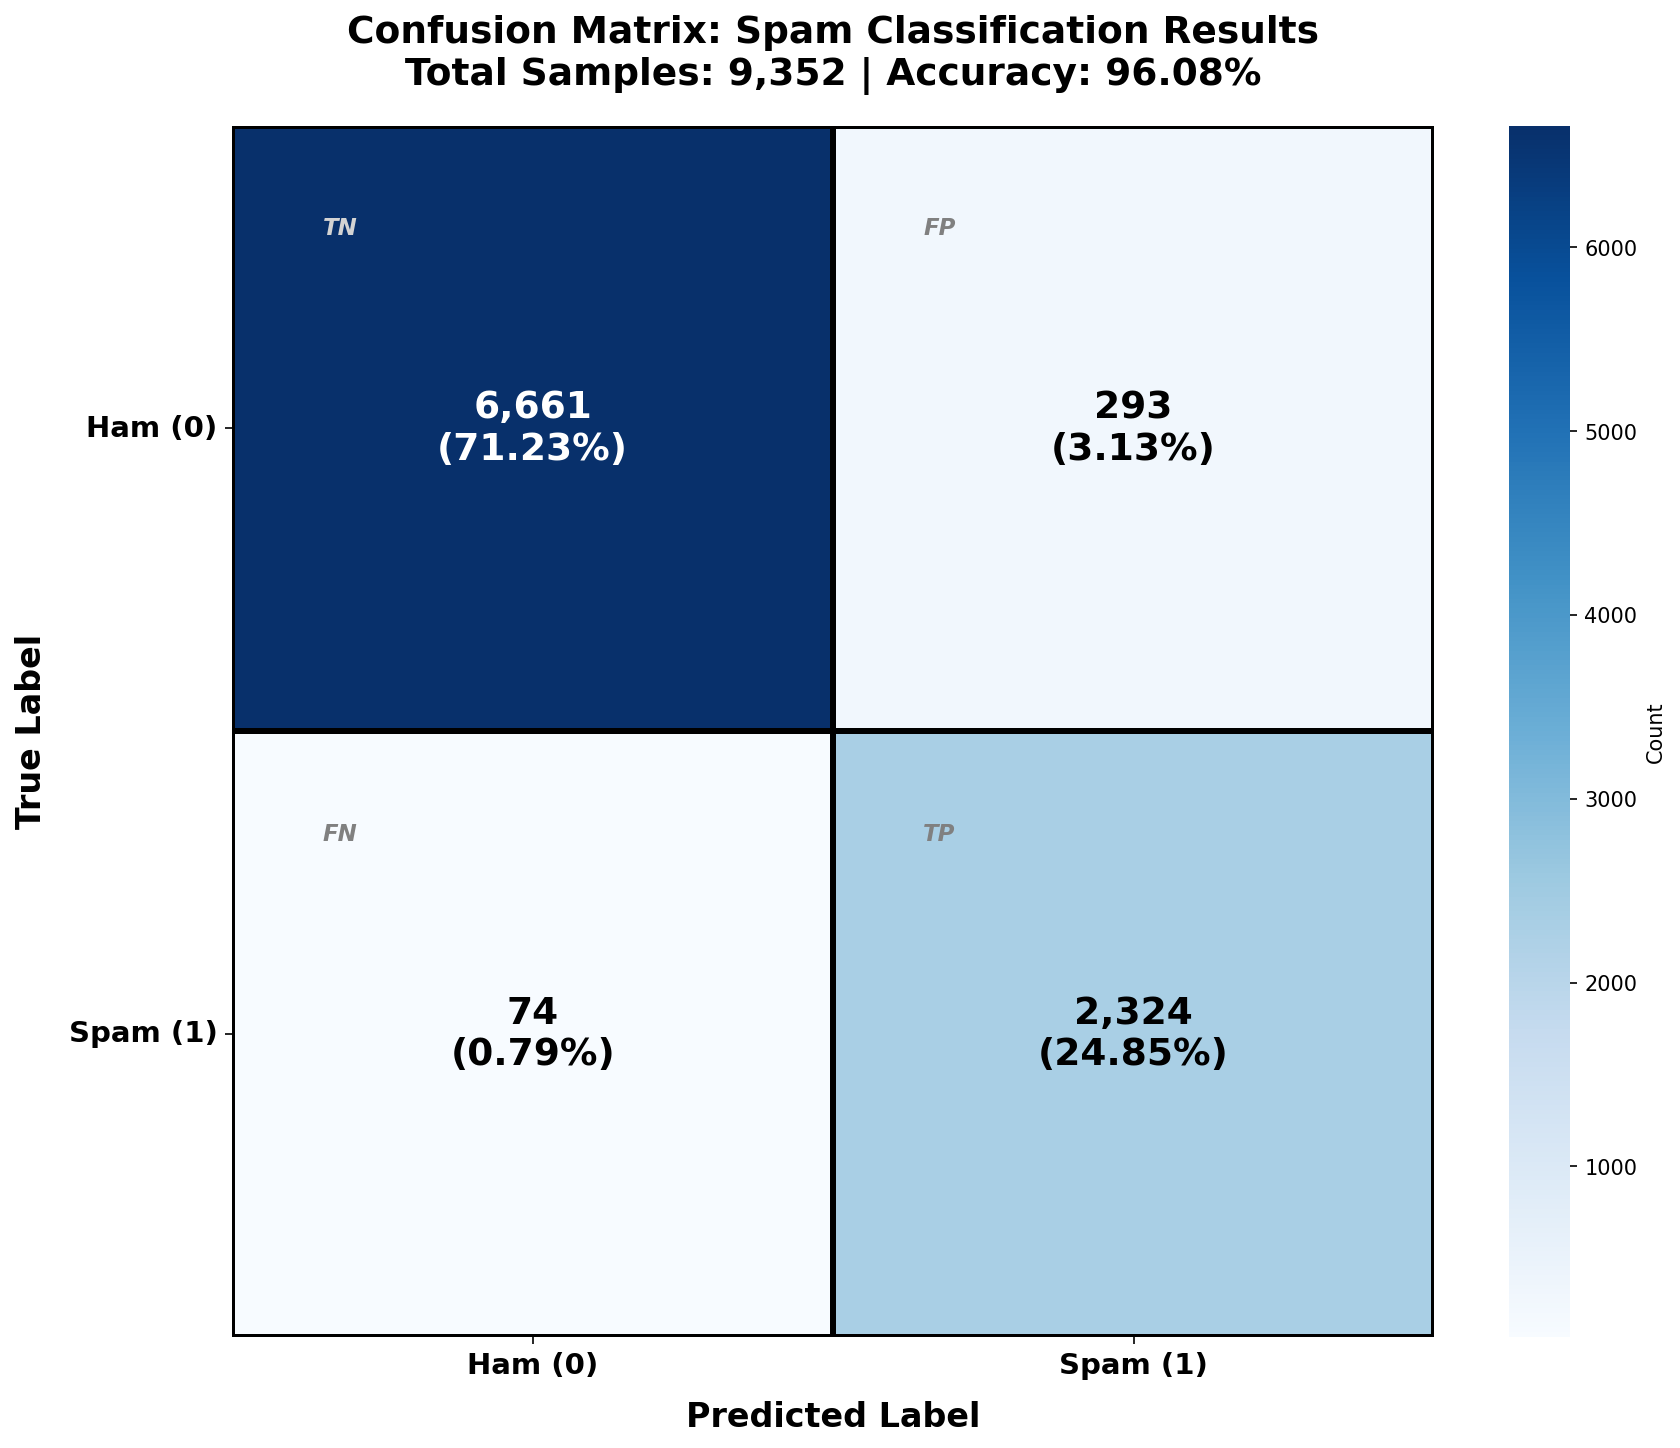
\includegraphics[width=0.75\textwidth]{04_confusion_matrix.png}
\caption{Confusion matrix for out-of-fold predictions over 100\% of the data (stratified 10-fold CV). Rows are true class; columns are predicted class. Counts and percentages are shown in each cell.}
\label{fig:confusion}
\end{figure}

\FloatBarrier

\paragraph{Decision threshold.} Adjusting the decision threshold alters the confusion matrix and metrics in predictable ways. Lowering the threshold (e.g., from 0.5 toward 0.3) increases the number of emails classified as spam, so recall for spam rises and false negatives fall, but false positives rise and precision for both classes typically falls. Raising the threshold reduces false positives and improves precision for ham at the cost of lower spam recall and more false negatives. Figure~\ref{fig:threshold} shows how accuracy, precision, and recall vary with threshold (and includes the ROC and precision--recall curves); the default 0.5 is near-optimal for overall accuracy and F1. ROC AUC is 0.9927, indicating strong separation of the two classes in probability space.

\begin{figure}[!htbp]
\centering
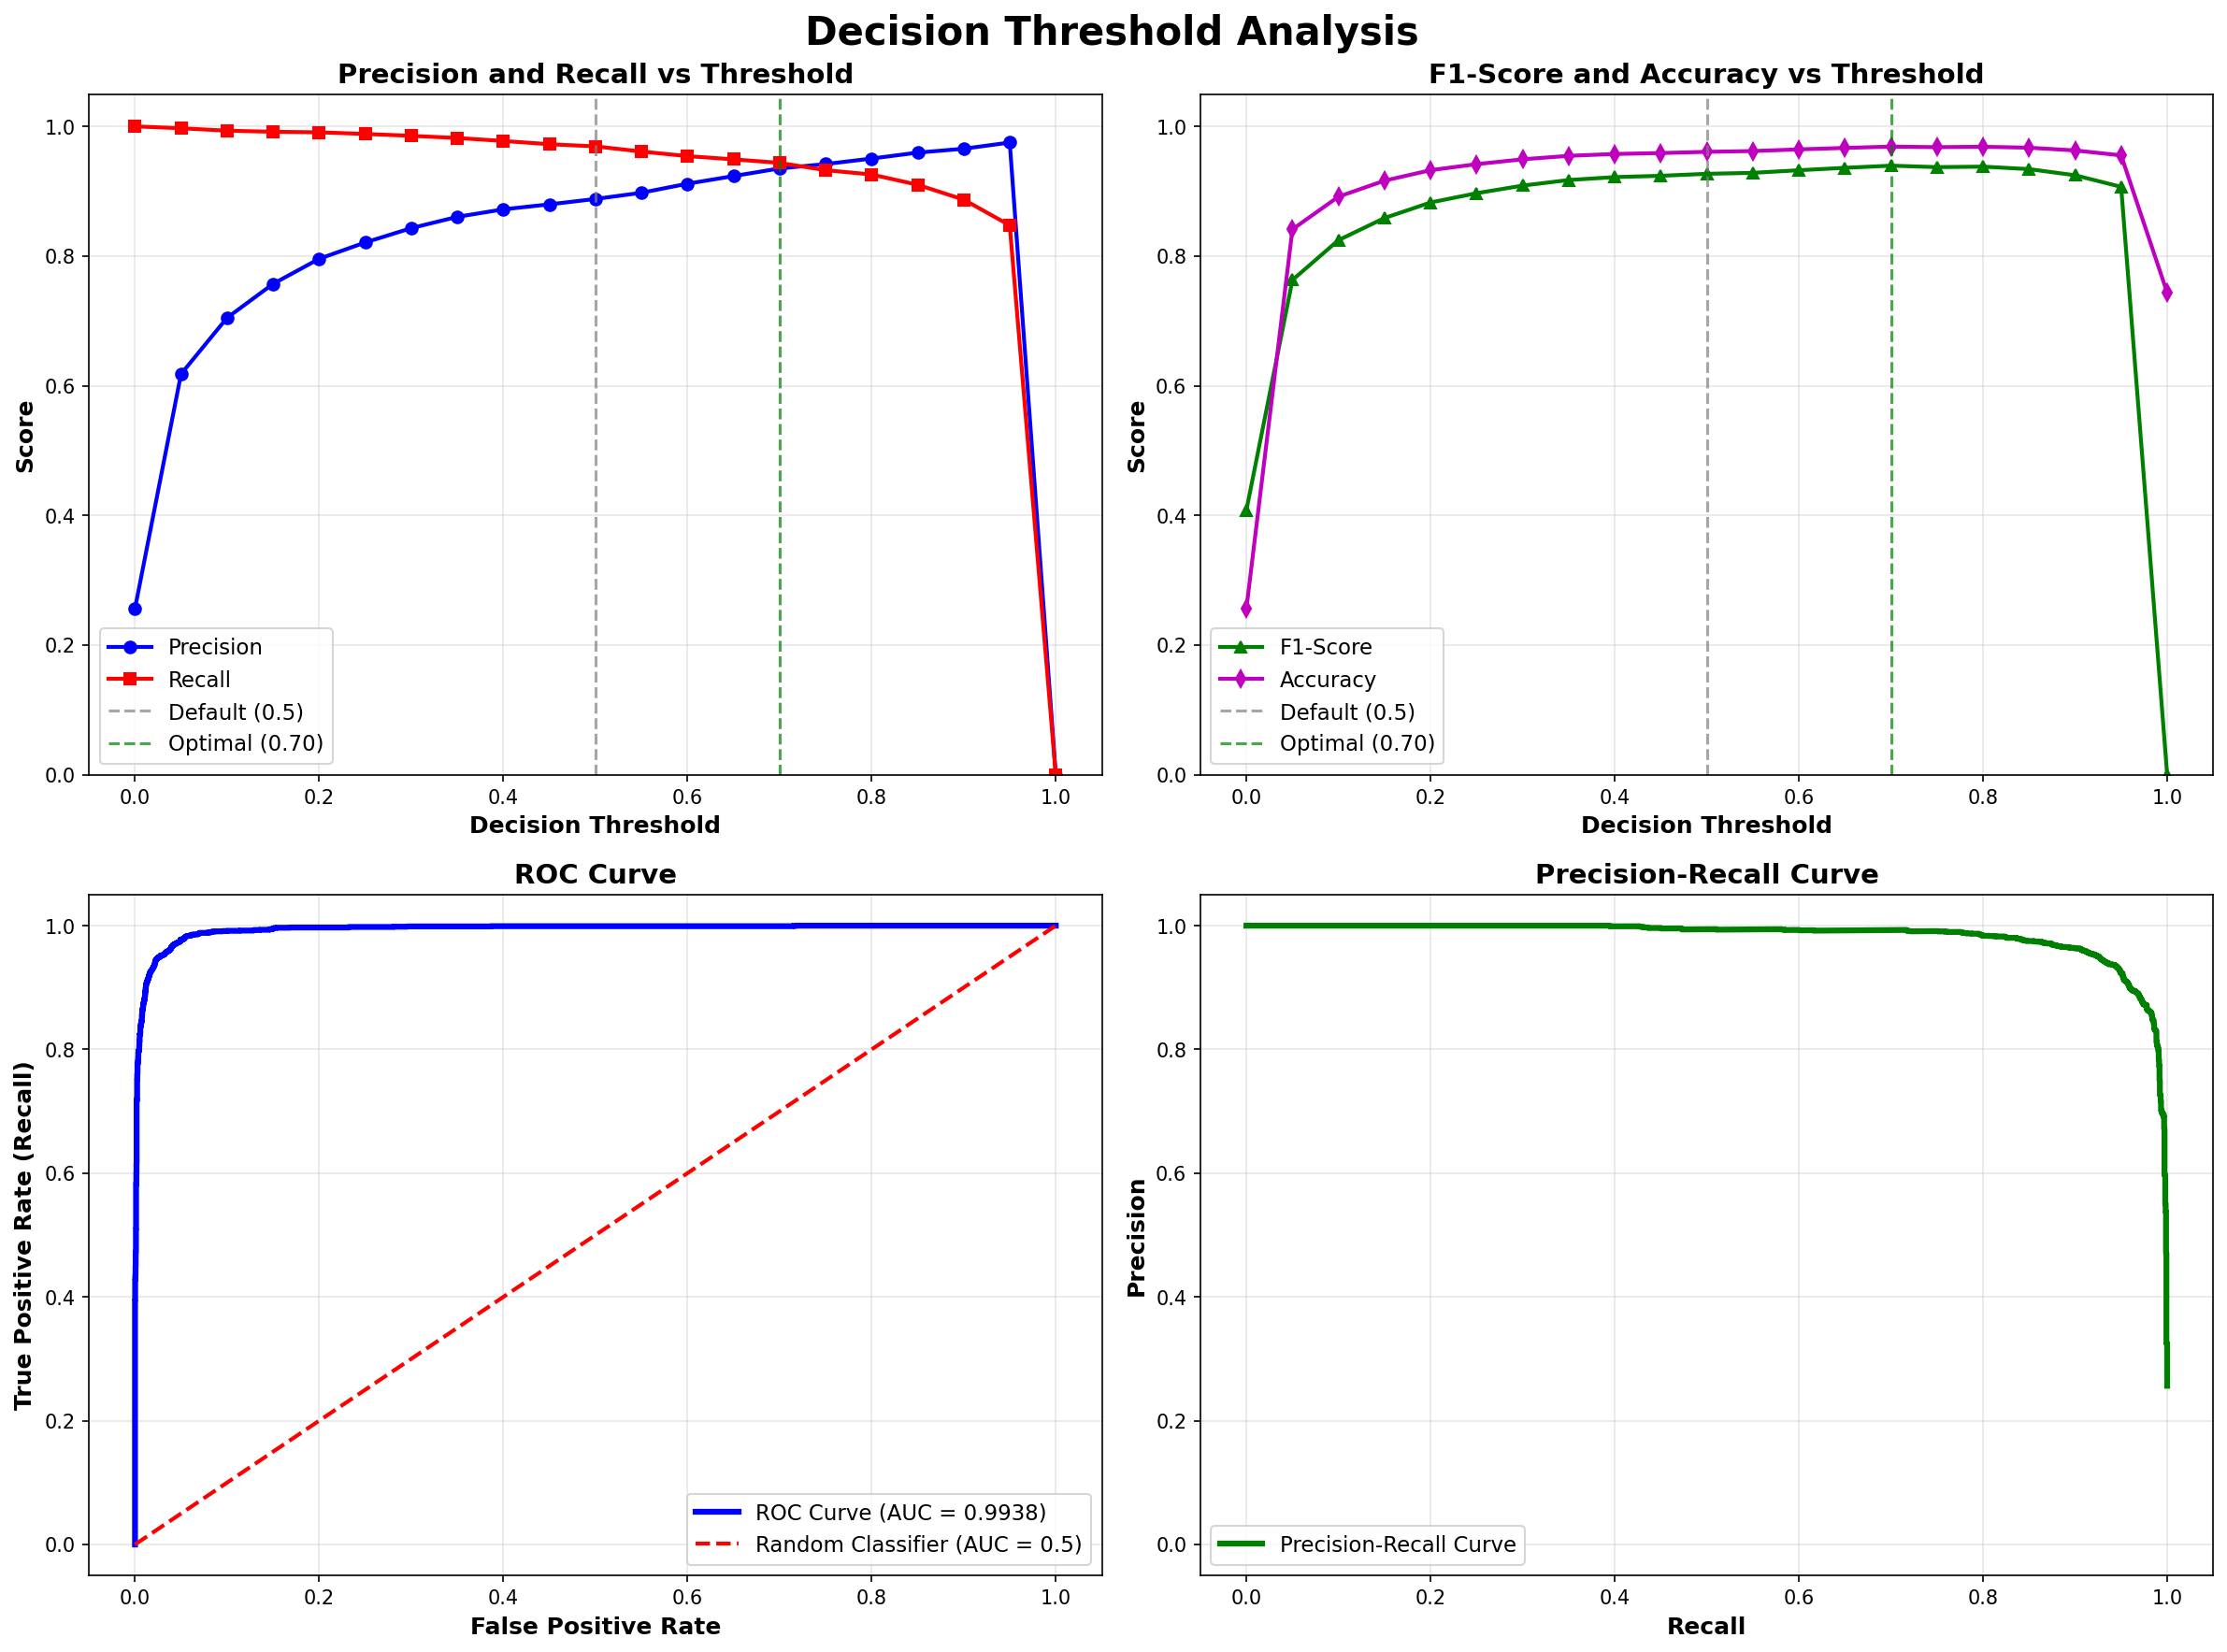
\includegraphics[width=0.85\textwidth]{05_threshold_analysis.png}
\caption{Decision threshold analysis: precision and recall vs.\ threshold (top left), F1 and accuracy vs.\ threshold (top right), ROC curve (bottom left), and precision--recall curve (bottom right).}
\label{fig:threshold}
\end{figure}

\FloatBarrier

\section{Discussion and Limitations}

The pipeline shows that Complement Naive Bayes with TF-IDF and cluster features achieves high accuracy and AUC. Algorithm choice mattered: Complement NB is better suited than standard Multinomial NB to the imbalanced setting. Clustering adds useful structure beyond raw vocabulary. The main limitations are the age and language of the corpus, the exclusion of metadata and non-text signals, and the static nature of the model (no continual adaptation to evolving spam).

\section{Conclusion}

This case study implemented and evaluated a spam classifier using Complement Naive Bayes on TF-IDF and cluster-derived features, validated by stratified 10-fold cross-validation. The model reaches 95.62\% accuracy with balanced precision and recall across classes. The design choices (Complement NB for imbalance, silhouette-based cluster count, and cross-validation without a separate test set) are documented and justified. The work demonstrates that classical, interpretable methods can perform well on spam classification when preprocessing and feature engineering are applied carefully.

\end{document}
